\documentclass[a4paper,12pt]{report}
\usepackage[utf8]{inputenc}
\usepackage{sectsty}
\usepackage{titlesec}
\titlelabel{\thetitle.\quad}
\setcounter{secnumdepth}{3}
\sectionfont{\normalsize}
\subsectionfont{\normalsize}
\usepackage{pdfpages}
\usepackage[table,xcdraw]{xcolor}
\usepackage{minted}
\renewcommand{\thechapter}{\Roman{chapter}\space }

\usepackage{titlesec}
\titleformat{\chapter}[display]
{\normalfont\large\bfseries}{\chaptertitlename\ \thechapter}{10pt}{\Large}  
\titlespacing{\chapter}{0pt}{0pt}{0pt}  

%=======================
% Adding the hyperref package for clickable links in ToC
\usepackage{hyperref}
\hypersetup{
    colorlinks=true,
    linkcolor=blue,
    urlcolor=blue,
    citecolor=blue,
    filecolor=blue
}

% Change "Chapter" to "Lab"
\renewcommand{\chaptername}{TP Embedded}

%----------------------------- MATLAB setup
\newcommand*{\underuparrow}[1]{\underset{\uparrow}{#1}}
\usepackage{listings}
\usepackage{xcolor}
\definecolor{codegreen}{rgb}{0,0.6,0}
\definecolor{codegray}{rgb}{0.5,0.5,0.5}
\definecolor{codepurple}{rgb}{0.58,0,0.82}
\definecolor{backcolour}{rgb}{54, 69, 79}
% ... (rest of the code setup)

\usepackage{geometry}
\geometry{bottom=2.5cm,top=2cm,left=2cm,right=2cm}
\usepackage{setspace}
%--------------------------------------

% Other packages...
\usepackage{amsfonts, amsmath, amssymb, amsthm}
\usepackage{tikz, tcolorbox}
\usepackage{enumitem}
\usepackage{tasks}
\usepackage{graphics}

\usepackage{graphicx}
\usepackage{float}
\usepackage{pgfplots}
\usepackage{tikz}
\usepackage{pgf-pie}
\usepackage[framemethod=TikZ]{mdframed}
\usepackage{wrapfig}
\usepackage{subcaption}
\renewcommand{\thesection}{\arabic{section}} 

% Setup for the table of contents
\usepackage{tocloft}
\chapternumberfont{\large} 
\chaptertitlefont{\Large}
\usepackage[mathscr]{euscript}
% ----------------------------------
% Define custom colors for syntax highlighting
\definecolor{keywordcolor}{rgb}{0.5, 0.5, 1}    % Light blue for keywords
\definecolor{commentcolor}{rgb}{0.4, 0.8, 0.4}  % Light green for comments
\definecolor{stringcolor}{rgb}{1, 0.6, 0.6}     % Light red for strings
\definecolor{framecolor}{rgb}{0.6, 0.6, 0.6}    % Gray frame

% Customize lstset with colors and appearance
\lstset{
    language=C,
    backgroundcolor=\color{white},              % Set background to white
    basicstyle=\ttfamily\footnotesize\color{black},  % Text in black
    keywordstyle=\bfseries\color{keywordcolor}, % Keyword color
    commentstyle=\itshape\color{commentcolor},  % Comment color
    stringstyle=\color{stringcolor},            % String color
    numbers=left,
    numberstyle=\tiny\color{gray},
    stepnumber=1,
    breaklines=true,
    frame=single,                               % Frame around the code
    rulecolor=\color{framecolor},               % Frame color
    tabsize=4,
    showspaces=false,
    showstringspaces=false
}
%----------------------------------

\title{Digital Circuit Design}
\author{KOY DANIEL}
\date{December 2022}
\pgfplotsset{compat=1.18}
\usepackage{chngcntr}
%\counterwithin{figure}{section}
\renewcommand\thefigure{\arabic{figure}}
\setcounter{figure}{0}
%-----------------------------------

% Page numbering and ToC setup
\begin{document}
% \includepdf[scale=1]{TP4.pdf}
% \includepdf[scale=1]{The Cover.pdf}
\pagenumbering{roman}
\onehalfspacing
\captionsetup{labelfont=bf}
\doublespacing
% \tableofcontents % Table of contents will now be clickable
% \addcontentsline{toc}{section}{\textbf{CONTENT}} % ToC linked
\singlespacing
\newpage
\pagenumbering{arabic}
\onehalfspacing
\chapter{ASSIGNMENT 1}
\par\noindent\rule{\textwidth}{0.4pt}%Draw line------

% -------------------------- INTRODUCTION ----------------------------------------------
\section{INTRODUCTION}
         \textbf{ESP32-C3 IoT Development Board}
         \begin{figure}[H]
             \centering
             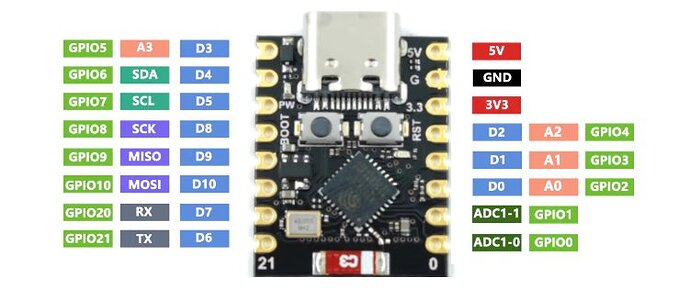
\includegraphics[width=0.7\linewidth]{ESP32-C3.png}
             \caption{ESP32-C3 and its Pinout}
             \label{fig:enter-label}
         \end{figure}
         The ESP32-C3 is a microcontroller with Wi-Fi and Bluetooth, commonly used in IoT projects. It can read data from analog, digital and I2C sensors. This report explains how to configure the ESP32-C3 to read these sensors, showing how each type can be used to gather environmental data for different applications. 
% --------------------------- SETUP DIAGRAM ---------------------------------------------
\section{SETUP DIAGRAM}
         This is the schematic of the setup connection:
         \begin{figure}[H]
             \centering
             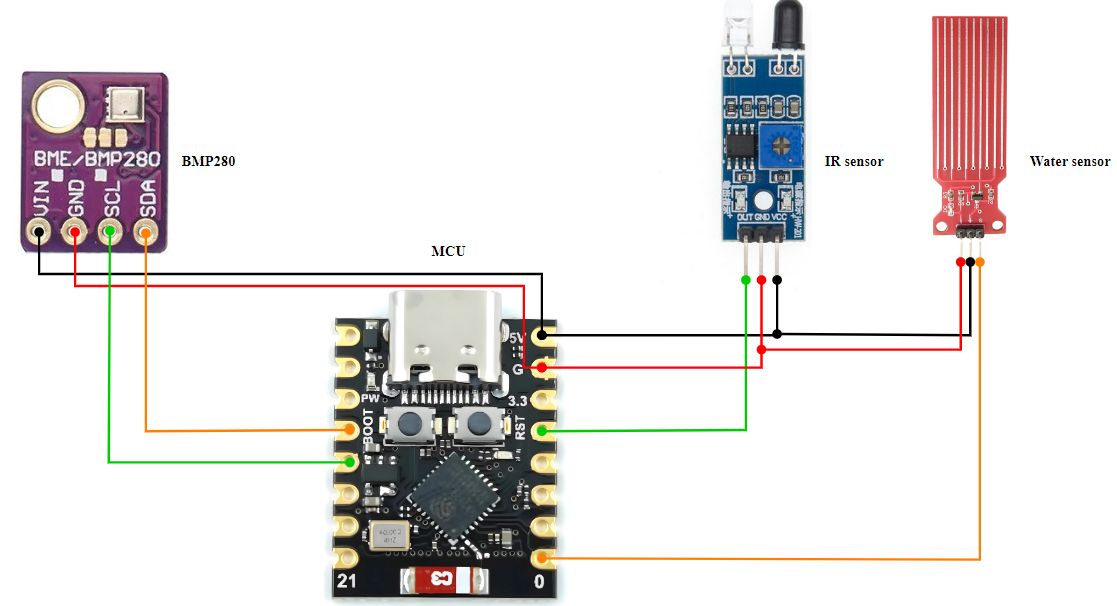
\includegraphics[width=0.7\linewidth]{setup.png}
             \caption{Setup diagram}
             \label{fig:enter-label}
         \end{figure}
         Here are the table of pin connections:
         \begin{table}[H]
         \caption{Pin Connection}
         \centering
         \renewcommand{\arraystretch}{1.5}
         \begin{tabular}{|c|l|}
         \hline
         Sensor       & \multicolumn{1}{c|}{Pin Connection}  \\ \hline
         BMP280       & VCC: 5V,  GND: G, SCL: Pin8, SDA: Pin9 \\ \hline
         IR Sensor    & VCC: 5V, GND: G, S: Pin0             \\ \hline
         Water Sensor & VCC: 5V, GND: G, OUT: Pin4           \\ \hline
         \end{tabular}
         \end{table}
         \begin{figure}[H]
             \centering
             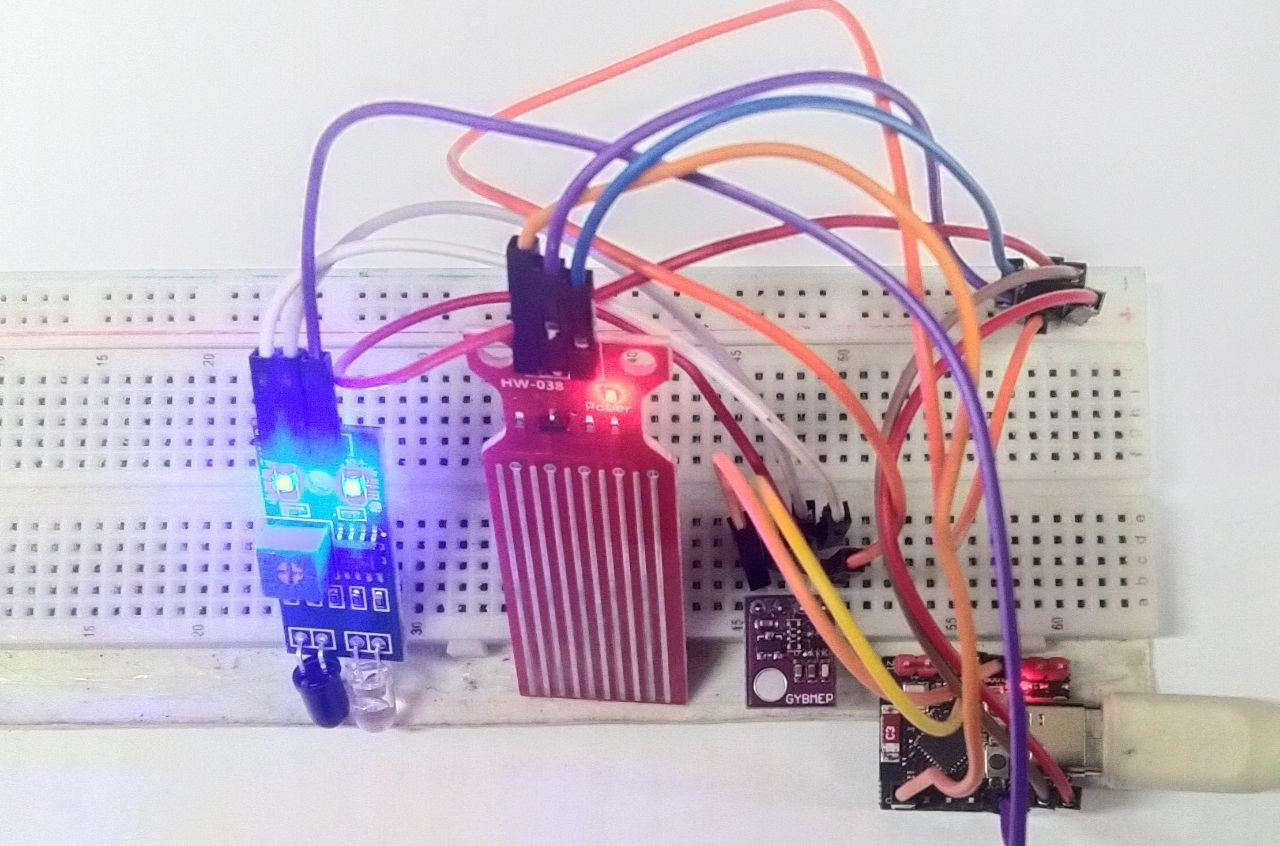
\includegraphics[width=0.7\linewidth]{set.png}
             \caption{Project setup}
             \label{fig:enter-label}
         \end{figure}
% --------------------------- CODE INTERPRETATION ---------------------------------------
\section{CODE INTERPRETATION}
         In this section we go through all the code. We read data from multiple sensors such as BMP280, the IR sensor, and the water sensor. So I will break the code to each sensor and the combination code you can find in my GitHub that is provided in the Appendix.
         \begin{enumerate}
             \item \textbf{ADC (Water Sensor)}
             \begin{lstlisting}
#define ADC_CHANNEL ADC_CHANNEL_0
const static char *TAG1 = "adc";
void ADC_Water_Sensor(void* param) {
    adc1_config_width(ADC_WIDTH_BIT_12);
    adc1_config_channel_atten(ADC_CHANNEL, ADC_ATTEN_DB_11);
    while (1) {
        int adc_reading = adc1_get_raw(ADC_CHANNEL);
        ESP_LOGI(TAG1, "ADC Value: %d\n", adc_reading);
        vTaskDelay(pdMS_TO_TICKS(1000));
    
    vTaskDelete(NULL);
}
             \end{lstlisting}
             \textbf{Explanation:}\\
             This part reads analog signals from a water sensor using the ADC of the ESP32. The ADC is configured for 12-bit resolution, and the raw data is logged every second. It demonstrates how to handle analog inputs for monitoring sensor values.
             \item \textbf{Digital Input (IR Sensor)}
             \begin{lstlisting}
#define IR_SENSOR_GPIO GPIO_NUM_4
const static char *TAG2 = "IR";
void DIGITAL_IR_Sensor(void* param) {
    gpio_config_t ir_config = {0};
    ir_config.mode = GPIO_MODE_INPUT;
    ir_config.pin_bit_mask = 1ULL << IR_SENSOR_GPIO;
    ir_config.pull_up_en = 0x0;
    ir_config.pull_down_en = 0x0;
    gpio_config(&ir_config);
    while (1) {
        int ir_state = gpio_get_level(IR_SENSOR_GPIO);
        ESP_LOGI(TAG2, "IR Sensor State: %s\n", ir_state ? "HIGH" : "LOW");
        vTaskDelay(pdMS_TO_TICKS(2000));
    }
    vTaskDelete(NULL);
}
             \end{lstlisting}
             \textbf{Explanation:}\\
             The IR sensor is connected to a GPIO pin, configured as an input. The code checks the pin state repeatedly to determine if the IR sensor detects an object (HIGH) or not (LOW). It showcases how to work with digital sensors.
             \item \textbf{I2C Communication (BMP280 Sensor)}
             \begin{enumerate}
                 \item \textbf{Initialization}
                 \begin{lstlisting}
void i2c_master_init() {
    i2c_config_t conf = {
        .mode = I2C_MODE_MASTER,
        .sda_io_num = I2C_MASTER_SDA_IO,
        .scl_io_num = I2C_MASTER_SCL_IO,
        .sda_pullup_en = GPIO_PULLUP_ENABLE,
        .scl_pullup_en = GPIO_PULLUP_ENABLE,
        .master.clk_speed = I2C_MASTER_FREQ_HZ,
    };
    i2c_param_config(I2C_MASTER_NUM, &conf);
    i2c_driver_install(I2C_MASTER_NUM, conf.mode, 0, 0, 0);
}
                 \end{lstlisting}
                 \item \textbf{Calibration Data}
                 \begin{lstlisting}
                     void bmp280_read_calibration() {
    uint8_t calib_raw[24];
    i2c_read(BMP280_REG_CALIB_START, calib_raw, 24);
    calib.T1 = (calib_raw[1] << 8) | calib_raw[0];
    calib.T2 = (calib_raw[3] << 8) | calib_raw[2];
    calib.T3 = (calib_raw[5] << 8) | calib_raw[4];
    // ...other calibration parameters...
}
                 \end{lstlisting}
                 \item \textbf{Reading and Compensating Temperature}
                 \begin{lstlisting}
int32_t bmp280_compensate_temperature(int32_t adc_T, int32_t *t_fine) {
    int32_t var1 = ((((adc_T >> 3) - ((int32_t)calib.T1 << 1))) * ((int32_t)calib.T2)) >> 11;
    int32_t var2 = (((((adc_T >> 4) - ((int32_t)calib.T1)) * ((adc_T >> 4) - ((int32_t)calib.T1))) >> 12) * ((int32_t)calib.T3)) >> 14;
    *t_fine = var1 + var2;
    return (*t_fine * 5 + 128) >> 8;
}
                 \end{lstlisting}
                 \item \textbf{Main Sensor Task}
                 \begin{lstlisting}
void I2C_BPM280(void* param) {
    i2c_master_init();
    bmp280_read_calibration();
    i2c_write(BMP280_REG_CTRL_MEAS, 0x27); // Configure sensor mode
    while (1) {
        uint8_t data[6];
        if (i2c_read(BMP280_REG_PRESS_MSB, data, 6) == ESP_OK) {
            int32_t adc_T = (data[3] << 12) | (data[4] << 4) | (data[5] >> 4);
            int32_t t_fine;
            int32_t temp = bmp280_compensate_temperature(adc_T, &t_fine);
            ESP_LOGI(TAG3, "Temperature: %.2f ^{o}C", temp / 100.0);
        } else {
            ESP_LOGE(TAG3, "Failed to read BMP280 data");
        }
    vTaskDelay(pdMS_TO_TICKS(3000));
    }
    vTaskDelete(NULL);
}
                 \end{lstlisting}
             \end{enumerate}
             \textbf{Explanation:}\\
             The I2C Communication (BMP280 Sensor) section sets up I2C communication with the BMP280 sensor, reads calibration data, and processes raw temperature readings using the sensor’s calibration values. The temperature is logged every three seconds, demonstrating real-time data collection with the ESP32.
             \item \textbf{Main Application}
             \begin{lstlisting}
void app_main() {
    xTaskCreate(I2C_BPM280, "BPM280", 2048, NULL, 5, NULL);
    xTaskCreate(DIGITAL_IR_Sensor, "IR_Sensor", 2048, NULL, 5, NULL);
    xTaskCreate(ADC_Water_Sensor, "Water_Sensor", 2048, NULL, 5, NULL);
}
             \end{lstlisting}
             \textbf{Explanation:}\\
             The \texttt{app\_main} function creates separate tasks for each sensor (ADC, IR, BMP280), allowing them to run concurrently without interfering with one another. It highlights multitasking using FreeRTOS.
         \end{enumerate}
% --------------------------- RESULT AND DISCUSSION -------------------------------------
\section{RESULT AND DISCUSSION}
         \begin{itemize}[label=$\blacksquare$]
             \item \textbf{Result}\\
             The log shows data from three sensors. The water sensor provides ADC values (26, 24, 25) with slight variation over time. The IR sensor state is LOW, meaning no object is detected. The BMP280 temperature sensor reports a temperature of 28.23°C. The ADC and IR sensor data are logged every 1000ms, while the BMP280 temperature is logged every 3000ms.
             \begin{figure}[H]
                 \centering
                 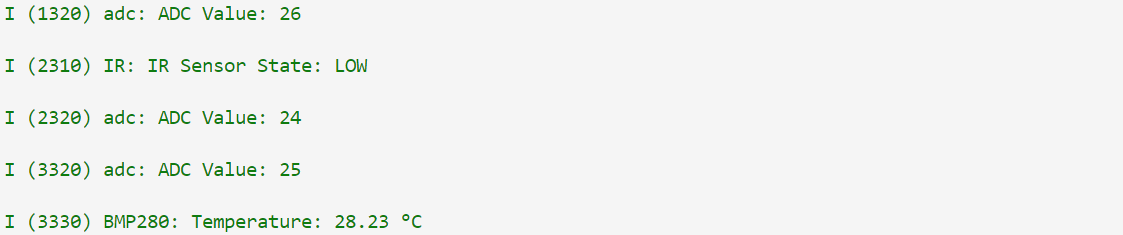
\includegraphics[width=0.8\linewidth]{result.png}
                 \caption{Result from the log message}
                 \label{fig:enter-label}
             \end{figure}
             \item \textbf{Discussion}\\
             From the result from the log message we can see that at each different time we receive the data from the sensor even though we set the priority the same but at different sampling time the output is still bias. If we want to see it clear we can use logic analyzer to see the pulse of each sensor.
         \end{itemize}
% --------------------------- CONCLUSION ------------------------------------------------
\section{CONCLUSION}
         In conclusion, this project demonstrates how the ESP32 interfaces with sensors using ADC, GPIO, and I2C. It focuses on teaching the use of \texttt{xTaskCreate} in FreeRTOS for real-time data collection and processing, laying the foundation for more advanced sensor-based systems.
% ---------------------------- APPENDIX -------------------------------------------------
\section{APPENDIX}
\textbf{GitHub} 
\end{document}

